%%%%%%%%%%%%%%%%%%%%%%%%%%%%%%%%%%%%%%%%%
%
% Important note:
% Chapter heading images should have a 2:1 width:height ratio,
% e.g. 920px width and 460px height.
%
% The original template (the Legrand Orange Book Template) can be found here --> http://www.latextemplates.com/template/the-legrand-orange-book
%
% Original author of the Legrand Orange Book Template:
% Mathias Legrand (legrand.mathias@gmail.com) with modifications by:
% Vel (vel@latextemplates.com)
%
% Original License:
% CC BY-NC-SA 3.0 (http://creativecommons.org/licenses/by-nc-sa/3.0/)
%%%%%%%%%%%%%%%%%%%%%%%%%%%%%%%%%%%%%%%%%
 
%----------------------------------------------------------------------------------------
%	PACKAGES AND OTHER DOCUMENT CONFIGURATIONS
%----------------------------------------------------------------------------------------

\documentclass[11pt,fleqn]{book} % Default font size and left-justified equations
\usepackage{hyperref}
\usepackage[top=3cm,bottom=3cm,left=3.2cm,right=3.2cm,headsep=10pt,letterpaper]{geometry} % Page margins
\usepackage[utf8]{inputenc}
\usepackage[english]{babel}
\usepackage{xcolor}
\usepackage[colorinlistoftodos]{todonotes}
\usepackage{xcolor} % Required for specifying colors by name
\definecolor{ocre}{RGB}{52,177,201} % Define the orange color used for highlighting throughout the book

% Font Settings
\usepackage{avant} % Use the Avantgarde font for headings
%\usepackage{times} % Use the Times font for headings
\usepackage{mathptmx} % Use the Adobe Times Roman as the default text font together with math symbols from the Sym­bol, Chancery and Com­puter Modern fonts

\usepackage{microtype} % Slightly tweak font spacing for aesthetics
\usepackage[utf8]{inputenc} % Required for including letters with accents
\usepackage[T1]{fontenc} % Use 8-bit encoding that has 256 glyphs

% Bibliography
\usepackage[style=alphabetic,sorting=nyt,sortcites=true,autopunct=true,babel=hyphen,hyperref=true,abbreviate=false,backref=true,backend=biber]{biblatex}
\addbibresource{bibliography.bib} % BibTeX bibliography file
\defbibheading{bibempty}{}
\hypersetup{
    colorlinks=true,
    linkcolor=blue,
    filecolor=magenta,      
    urlcolor=cyan,
}

\urlstyle{same}


%%%%%%%%%%%%%%%%%%%%%%%%%%%%%%%%%%%%%%%%%
% This is based on the Legrand Orange Book
% Structural Definitions File
%
% The original template (the Legrand Orange Book Template) can be found here --> http://www.latextemplates.com/template/the-legrand-orange-book
%
% Original author of the Legrand Orange Book Template::
% Mathias Legrand (legrand.mathias@gmail.com) with modifications by:
% Vel (vel@latextemplates.com)
%
% Original License:
% CC BY-NC-SA 3.0 (http://creativecommons.org/licenses/by-nc-sa/3.0/)
%
%%%%%%%%%%%%%%%%%%%%%%%%%%%%%%%%%%%%%%%%%
%----------------------------------------------------------------------------------------
%	VARIOUS REQUIRED PACKAGES
%----------------------------------------------------------------------------------------

\usepackage{titlesec} % Allows customization of titles

\usepackage{graphicx} % Required for including pictures
\graphicspath{{Pictures/}} % Specifies the directory where pictures are stored

\usepackage{lipsum} % Inserts dummy text

\usepackage{tikz} % Required for drawing custom shapes

\usepackage[english]{babel} % English language/hyphenation

\usepackage{enumitem} % Customize lists
\setlist{nolistsep} % Reduce spacing between bullet points and numbered lists

\usepackage{booktabs} % Required for nicer horizontal rules in tables

\usepackage{eso-pic} % Required for specifying an image background in the title page

%----------------------------------------------------------------------------------------
%	MAIN TABLE OF CONTENTS
%----------------------------------------------------------------------------------------

\usepackage{titletoc} % Required for manipulating the table of contents

\contentsmargin{0cm} % Removes the default margin
% Chapter text styling
\titlecontents{chapter}[1.25cm] % Indentation
{\addvspace{15pt}\large\sffamily\bfseries} % Spacing and font options for chapters
{\color{ocre!60}\contentslabel[\Large\thecontentslabel]{1.25cm}\color{ocre}} % Chapter number
{}  
{\color{ocre!60}\normalsize\sffamily\bfseries\;\titlerule*[.5pc]{.}\;\thecontentspage} % Page number
% Section text styling
\titlecontents{section}[1.25cm] % Indentation
{\addvspace{5pt}\sffamily\bfseries} % Spacing and font options for sections
{\contentslabel[\thecontentslabel]{1.25cm}} % Section number
{}
{\sffamily\hfill\color{black}\thecontentspage} % Page number
[]
% Subsection text styling
\titlecontents{subsection}[1.25cm] % Indentation
{\addvspace{1pt}\sffamily\small} % Spacing and font options for subsections
{\contentslabel[\thecontentslabel]{1.25cm}} % Subsection number
{}
{\sffamily\;\titlerule*[.5pc]{.}\;\thecontentspage} % Page number
[] 

%----------------------------------------------------------------------------------------
%	MINI TABLE OF CONTENTS IN CHAPTER HEADS
%----------------------------------------------------------------------------------------

% Section text styling
\titlecontents{lsection}[0em] % Indendating
{\footnotesize\sffamily} % Font settings
{}
{}
{}

% Subsection text styling
\titlecontents{lsubsection}[.5em] % Indentation
{\normalfont\footnotesize\sffamily} % Font settings
{}
{}
{}
 
%----------------------------------------------------------------------------------------
%	PAGE HEADERS
%----------------------------------------------------------------------------------------

\usepackage{fancyhdr} % Required for header and footer configuration

\pagestyle{fancy}
\renewcommand{\chaptermark}[1]{\markboth{\sffamily\normalsize\bfseries\chaptername\ \thechapter.\ #1}{}} % Chapter text font settings
\renewcommand{\sectionmark}[1]{\markright{\sffamily\normalsize\thesection\hspace{5pt}#1}{}} % Section text font settings
\fancyhf{} \fancyhead[LE,RO]{\sffamily\normalsize\thepage} % Font setting for the page number in the header
\fancyhead[RE]{\leftmark} % Print the current chapter name on the right side of even pages
\renewcommand{\headrulewidth}{0.5pt} % Width of the rule under the header
\addtolength{\headheight}{2.5pt} % Increase the spacing around the header slightly
\renewcommand{\footrulewidth}{0pt} % Removes the rule in the footer
\fancypagestyle{plain}{\fancyhead{}\renewcommand{\headrulewidth}{0pt}} % Style for when a plain pagestyle is specified

% Removes the header from odd empty pages at the end of chapters
\makeatletter
\renewcommand{\cleardoublepage}{
\clearpage\ifodd\c@page\else
\hbox{}
\vspace*{\fill}
\thispagestyle{empty}
\newpage
\fi}
%----------------------------------------------------------------------------------------
%	THEOREM STYLES
%----------------------------------------------------------------------------------------

\usepackage{amsmath,amsfonts,amssymb,amsthm} % For math equations, theorems, symbols, etc

\newcommand{\intoo}[2]{\mathopen{]}#1\,;#2\mathclose{[}}
\newcommand{\ud}{\mathop{\mathrm{{}d}}\mathopen{}}
\newcommand{\intff}[2]{\mathopen{[}#1\,;#2\mathclose{]}}
\newtheorem{notation}{Notation}[chapter]

%%%%%%%%%%%%%%%%%%%%%%%%%%%%%%%%%%%%%%%%%%%%%%%%%%%%%%%%%%%%%%%%%%%%%%%%%%%
%%%%%%%%%%%%%%%%%%%% dedicated to boxed/framed environements %%%%%%%%%%%%%%
%%%%%%%%%%%%%%%%%%%%%%%%%%%%%%%%%%%%%%%%%%%%%%%%%%%%%%%%%%%%%%%%%%%%%%%%%%%
\newtheoremstyle{ocrenumbox}% % Theorem style name
{0pt}% Space above
{0pt}% Space below
{\normalfont}% % Body font
{}% Indent amount
{\small\bf\sffamily\color{ocre}}% % Theorem head font
{\;}% Punctuation after theorem head
{0.25em}% Space after theorem head
{\small\sffamily\color{ocre}\thmname{#1}\nobreakspace\thmnumber{\@ifnotempty{#1}{}\@upn{#2}}% Theorem text (e.g. Theorem 2.1)
\thmnote{\nobreakspace\the\thm@notefont\sffamily\bfseries\color{black}---\nobreakspace#3.}} % Optional theorem note
\renewcommand{\qedsymbol}{$\blacksquare$}% Optional qed square

\newtheoremstyle{blacknumex}% Theorem style name
{5pt}% Space above
{5pt}% Space below
{\normalfont}% Body font
{} % Indent amount
{\small\bf\sffamily}% Theorem head font
{\;}% Punctuation after theorem head
{0.25em}% Space after theorem head
{\small\sffamily{\tiny\ensuremath{\blacksquare}}\nobreakspace\thmname{#1}\nobreakspace\thmnumber{\@ifnotempty{#1}{}\@upn{#2}}% Theorem text (e.g. Theorem 2.1)
\thmnote{\nobreakspace\the\thm@notefont\sffamily\bfseries---\nobreakspace#3.}}% Optional theorem note

\newtheoremstyle{blacknumbox} % Theorem style name
{0pt}% Space above
{0pt}% Space below
{\normalfont}% Body font
{}% Indent amount
{\small\bf\sffamily}% Theorem head font
{\;}% Punctuation after theorem head
{0.25em}% Space after theorem head
{\small\sffamily\thmname{#1}\nobreakspace\thmnumber{\@ifnotempty{#1}{}\@upn{#2}}% Theorem text (e.g. Theorem 2.1)
\thmnote{\nobreakspace\the\thm@notefont\sffamily\bfseries---\nobreakspace#3.}}% Optional theorem note

%%%%%%%%%%%%%%%%%%%%%%%%%%%%%%%%%%%%%%%%%%%%%%%%%%%%%%%%%%%%%%%%%%%%%%%%%%%
%%%%%%%%%%%%% dedicated to non-boxed/non-framed environements %%%%%%%%%%%%%
%%%%%%%%%%%%%%%%%%%%%%%%%%%%%%%%%%%%%%%%%%%%%%%%%%%%%%%%%%%%%%%%%%%%%%%%%%%
\newtheoremstyle{ocrenum}% % Theorem style name
{5pt}% Space above
{5pt}% Space below
{\normalfont}% % Body font
{}% Indent amount
{\small\bf\sffamily\color{ocre}}% % Theorem head font
{\;}% Punctuation after theorem head
{0.25em}% Space after theorem head
{\small\sffamily\color{ocre}\thmname{#1}\nobreakspace\thmnumber{\@ifnotempty{#1}{}\@upn{#2}}% Theorem text (e.g. Theorem 2.1)
\thmnote{\nobreakspace\the\thm@notefont\sffamily\bfseries\color{black}---\nobreakspace#3.}} % Optional theorem note
\renewcommand{\qedsymbol}{$\blacksquare$}% Optional qed square
\makeatother

% Defines the theorem text style for each type of theorem to one of the three styles above
\newcounter{dummy} 
\numberwithin{dummy}{section}
\theoremstyle{ocrenumbox}
\newtheorem{theoremeT}[dummy]{Theorem}
\newtheorem{problem}{Problem}[chapter]
\newtheorem{exerciseT}{Exercise}[chapter]
\theoremstyle{blacknumex}
\newtheorem{exampleT}{Example}[chapter]
\theoremstyle{blacknumbox}
\newtheorem{vocabulary}{Vocabulary}[chapter]
\newtheorem{definitionT}{Definition}[section]
\newtheorem{corollaryT}[dummy]{Corollary}
\theoremstyle{ocrenum}
\newtheorem{proposition}[dummy]{Proposition}

%----------------------------------------------------------------------------------------
%	DEFINITION OF COLORED BOXES
%----------------------------------------------------------------------------------------

\RequirePackage[framemethod=default]{mdframed} % Required for creating the theorem, definition, exercise and corollary boxes

% Theorem box
\newmdenv[skipabove=7pt,
skipbelow=7pt,
backgroundcolor=black!5,
linecolor=ocre,
innerleftmargin=5pt,
innerrightmargin=5pt,
innertopmargin=5pt,
leftmargin=0cm,
rightmargin=0cm,
innerbottommargin=5pt]{tBox}

% Exercise box	  
\newmdenv[skipabove=7pt,
skipbelow=7pt,
rightline=false,
leftline=true,
topline=false,
bottomline=false,
backgroundcolor=ocre!10,
linecolor=ocre,
innerleftmargin=5pt,
innerrightmargin=5pt,
innertopmargin=5pt,
innerbottommargin=5pt,
leftmargin=0cm,
rightmargin=0cm,
linewidth=4pt]{eBox}	

% Definition box
\newmdenv[skipabove=7pt,
skipbelow=7pt,
rightline=false,
leftline=true,
topline=false,
bottomline=false,
linecolor=ocre,
innerleftmargin=5pt,
innerrightmargin=5pt,
innertopmargin=0pt,
leftmargin=0cm,
rightmargin=0cm,
linewidth=4pt,
innerbottommargin=0pt]{dBox}	

% Corollary box
\newmdenv[skipabove=7pt,
skipbelow=7pt,
rightline=false,
leftline=true,
topline=false,
bottomline=false,
linecolor=gray,
backgroundcolor=black!5,
innerleftmargin=5pt,
innerrightmargin=5pt,
innertopmargin=5pt,
leftmargin=0cm,
rightmargin=0cm,
linewidth=4pt,
innerbottommargin=5pt]{cBox}

% Creates an environment for each type of theorem and assigns it a theorem text style from the "Theorem Styles" section above and a colored box from above
\newenvironment{theorem}{\begin{tBox}\begin{theoremeT}}{\end{theoremeT}\end{tBox}}
\newenvironment{exercise}{\begin{eBox}\begin{exerciseT}}{\hfill{\color{ocre}\tiny\ensuremath{\blacksquare}}\end{exerciseT}\end{eBox}}				  
\newenvironment{definition}{\begin{dBox}\begin{definitionT}}{\end{definitionT}\end{dBox}}	
\newenvironment{example}{\begin{exampleT}}{\hfill{\tiny\ensuremath{\blacksquare}}\end{exampleT}}		
\newenvironment{corollary}{\begin{cBox}\begin{corollaryT}}{\end{corollaryT}\end{cBox}}	

%----------------------------------------------------------------------------------------
%	REMARK ENVIRONMENT
%----------------------------------------------------------------------------------------

\newenvironment{remark}{\par\vspace{10pt}\small % Vertical white space above the remark and smaller font size
\begin{list}{}{
\leftmargin=35pt % Indentation on the left
\rightmargin=25pt}\item\ignorespaces % Indentation on the right
\makebox[-2.5pt]{\begin{tikzpicture}[overlay]
\node[draw=ocre!60,line width=1pt,circle,fill=ocre!25,font=\sffamily\bfseries,inner sep=2pt,outer sep=0pt] at (-15pt,0pt){\textcolor{ocre}{R}};\end{tikzpicture}} % Orange R in a circle
\advance\baselineskip -1pt}{\end{list}\vskip5pt} % Tighter line spacing and white space after remark

%----------------------------------------------------------------------------------------
%	SECTION NUMBERING IN THE MARGIN
%----------------------------------------------------------------------------------------

\makeatletter
\renewcommand{\@seccntformat}[1]{\llap{\textcolor{ocre}{\csname the#1\endcsname}\hspace{1em}}}                    
\renewcommand{\section}{\@startsection{section}{1}{\z@}
{-4ex \@plus -1ex \@minus -.4ex}
{1ex \@plus.2ex }
{\normalfont\large\sffamily\bfseries}}
\renewcommand{\subsection}{\@startsection {subsection}{2}{\z@}
{-3ex \@plus -0.1ex \@minus -.4ex}
{0.5ex \@plus.2ex }
{\normalfont\sffamily\bfseries}}
\renewcommand{\subsubsection}{\@startsection {subsubsection}{3}{\z@}
{-2ex \@plus -0.1ex \@minus -.2ex}
{.2ex \@plus.2ex }
{\normalfont\small\sffamily\bfseries}}                        
\renewcommand\paragraph{\@startsection{paragraph}{4}{\z@}
{-2ex \@plus-.2ex \@minus .2ex}
{.1ex}
{\normalfont\small\sffamily\bfseries}}

%----------------------------------------------------------------------------------------
%	HYPERLINKS IN THE DOCUMENTS
%----------------------------------------------------------------------------------------

% For an unclear reason, the package should be loaded now and not later
\usepackage{hyperref}
\hypersetup{hidelinks,backref=true,pagebackref=true,hyperindex=true,colorlinks=false,breaklinks=true,urlcolor= ocre,bookmarks=true,bookmarksopen=false,pdftitle={Title},pdfauthor={Author}}

%----------------------------------------------------------------------------------------
%	CHAPTER HEADINGS
%----------------------------------------------------------------------------------------

% The set-up below should be (sadly) manually adapted to the overall margin page septup controlled by the geometry package loaded in the main.tex document. It is possible to implement below the dimensions used in the goemetry package (top,bottom,left,right)... TO BE DONE

\newcommand{\thechapterimage}{}
\newcommand{\chapterimage}[1]{\renewcommand{\thechapterimage}{#1}}

% Numbered chapters with mini tableofcontents
\def\thechapter{\arabic{chapter}}
\def\@makechapterhead#1{
\thispagestyle{empty}
{\centering \normalfont\sffamily
\ifnum \c@secnumdepth >\m@ne
\if@mainmatter
\startcontents
\begin{tikzpicture}[remember picture,overlay]
\node at (current page.north west)
{\begin{tikzpicture}[remember picture,overlay]
\node[anchor=north west,inner sep=0pt] at (0,0) {\includegraphics[width=\paperwidth]{\thechapterimage}};
%%%%%%%%%%%%%%%%%%%%%%%%%%%%%%%%%%%%%%%%%%%%%%%%%%%%%%%%%%%%%%%%%%%%%%%%%%%%%%%%%%%%%
% Commenting the 3 lines below removes the small contents box in the chapter heading
%\fill[color=ocre!10!white,opacity=.6] (1cm,0) rectangle (8cm,-7cm);
%\node[anchor=north west] at (1.1cm,.35cm) {\parbox[t][8cm][t]{6.5cm}{\huge\bfseries\flushleft \printcontents{l}{1}{\setcounter{tocdepth}{2}}}};
\draw[anchor=west] (5cm,-9cm) node [rounded corners=20pt,fill=ocre!10!white,text opacity=1,draw=ocre,draw opacity=1,line width=1.5pt,fill opacity=.6,inner sep=12pt]{\huge\sffamily\bfseries\textcolor{black}{\thechapter. #1\strut\makebox[22cm]{}}};
%%%%%%%%%%%%%%%%%%%%%%%%%%%%%%%%%%%%%%%%%%%%%%%%%%%%%%%%%%%%%%%%%%%%%%%%%%%%%%%%%%%%%
\end{tikzpicture}};
\end{tikzpicture}}
\par\vspace*{230\p@}
\fi
\fi}

% Unnumbered chapters without mini tableofcontents (could be added though) 
\def\@makeschapterhead#1{
\thispagestyle{empty}
{\centering \normalfont\sffamily
\ifnum \c@secnumdepth >\m@ne
\if@mainmatter
\begin{tikzpicture}[remember picture,overlay]
\node at (current page.north west)
{\begin{tikzpicture}[remember picture,overlay]
\node[anchor=north west,inner sep=0pt] at (0,0) {\includegraphics[width=\paperwidth]{\thechapterimage}};
\draw[anchor=west] (5cm,-9cm) node [rounded corners=20pt,fill=ocre!10!white,fill opacity=.6,inner sep=12pt,text opacity=1,draw=ocre,draw opacity=1,line width=1.5pt]{\huge\sffamily\bfseries\textcolor{black}{#1\strut\makebox[22cm]{}}};
\end{tikzpicture}};
\end{tikzpicture}}
\par\vspace*{230\p@}
\fi
\fi
}
\makeatother % Insert the commands.tex file which contains the majority of the structure behind the template

\begin{document}
\title{Introduction to REALTA}

%----------------------------------------------------------------------------------------
%	TITLE PAGE
%----------------------------------------------------------------------------------------

\begingroup
\thispagestyle{empty}
\AddToShipoutPicture*{\put(0,0){
\includegraphics[scale=1.25]{esahubble}}} % Image background
\centering
\vspace*{5cm}
\par\normalfont\fontsize{35}{35}\sffamily\selectfont
\textbf{Introduction to REALTA}\\
{\LARGE A User Guide for I-LOFAR Computer System}\par % Book title
\vspace*{1cm}
{\Huge Aoife Brennan}\par % Author name
\endgroup

%----------------------------------------------------------------------------------------
%	COPYRIGHT PAGE
%----------------------------------------------------------------------------------------

\newpage
~\vfill
\thispagestyle{empty}
\noindent \textsc{Summer Research Internship, I-LOFAR, Birr, Ireland}\\



\noindent This user guide was written as part of a larger summer project under the supervision of Dr. Evan Keane with the financial support of the I-LOFAR and  BreakThrough Listen Project, Berkeley. \\ % License information


\todo[inline, color=green!20]{the image on the cover is a Hubble image, this will be changed to something more suitable later.}%
\noindent \textit{First release, July 2020} % Printing/edition date


%----------------------------------------------------------------------------------------
%	TABLE OF CONTENTS
%----------------------------------------------------------------------------------------


\pagestyle{empty} % No headers

\tableofcontents % Print the table of contents itself
\todo[size=\small, color=green!20]{I also wanted to write a section including what happens to raw data after observing.}%
%\cleardoublepage % Forces the first chapter to start on an odd page so it's on the right

\pagestyle{fancy} % Print headers again

%----------------------------------------------------------------------------------------
%	CHAPTER 1
%----------------------------------------------------------------------------------------

\chapterimage{header.png} % Chapter heading image


\section{Overview}



I-LOFAR is an Irish radio observatory, a part of a more extensive network of telescopes observing at low radio frequency (10 – 240) Mhz, collectively referred to as LOFAR. REALTA is the backend system for I-LOFAR and can be used as a gateway to connect to the I-LOFAR observing array, via (ucc1). REALTA is composed of four nodes (ucc1, ucc2, ucc3, and ucc4), all of which are mounted on. The first node (ucc1) is used for running observing scripts, acting as a connection between the physical observing system and data processing nodes. After observing using (ucc1), data can then be transferred from (ucc1) to the data processing nodes (ucc2, ucc3, ucc4). Many different data files can be produced when observing with I-LOFAR and processed by scripts written in many different languages. Furthermore, many different data processing softwares are installed, frequently in the form of dockers.
The following user guide is divided into nine sections, as listed in contents. 

Section two describes how to access REALTA, by ssh into the REALTA gateway. Section three describes the general structure of the I-LOFAR computer system, giving an overview of the system's back end. Section four gives a brief guide to navigating processing nodes using simple bash commands. Section five describes the usage of dockers on REALTA. Section six demonstrates useful data processing commands with applications. Section seven gives an example of an observing script, along with a general methodology for observing in (ucc1). Section eight contains a sample data processing script. Section nine gives resources to software guides and command references that are useful when using REALTA.

\section{Accessing REALTA}
The easiest way to access REALTA is to ssh into the gateway from either a Mac or Linux operating system. Before accessing REALTA on a Windows system, a terminal like program must be installed, resources for windows are listed in section five. The command terminal for both a Mac or Linux operating system will work. REALTA can is accessible by using the ssh command to access the Linux gateway @lgc.lofar.dias.ie. First, a whitelisted IvP4 must be obtained the IvP4 used must be stable and pingable. After whitelisting an IvP4, a username and password will be assigned.  The command below demonstrates how to ssh into REALTA, where username is the unique username assigned after whitelisting.

\vspace{3mm}

\verb|$ ssh username@160.6.237.10|

\vspace{3mm}

In order to access REALTA in a more timely manner a public key can be generated, this can be used to authenticate the user without entering a password when logging in. An alias can also be used, to shorten the command used to ssh into REALTA from our first command example to a shorten command as follows,

\vspace{3mm}
\verb|$ ssh lgc|
\vspace{3mm}

Resources for creating and using both aliases and public keys and listed in section nine.


\section{I-LOFAR Computer System}
I-LOFAR consists of two different types of array, the low band array (LBA) which observes in the range of 10 MHz to 90 Mhz, and consists of an array of pole like antennas. The second array, the high band array (HBA), observes in the range 110 MHz to 240 Mhz. The (HBA) array consists of a series of tile-like antennas. The input signals from the (LBA) and (HBA) arrays are transported by coaxial cables, to the receiver control unit (RCU) which is located in the I-LOFAR cabinet. The receiver unit performs input selection, then the signal is amplified and filtered by a A/D converter. After this, the signal goes into the remote station processing board (RSP). In the (RSP), the signal goes into a first in first out buffer (FIFO). Then goes through a polyphase filter, which is a fast Fourier transform implementation of a bandpass filter bank. The filter makes the signal bandwidth small enough for beamforming to take place. In addition to beamforming, the RSP boards can calculate subband statistics, beamlet statistics, and array covariances. 

The Transient buffer boards (TBB) are not part of the main signal processing chain, but their function is to store a short period of raw voltage data. The first two components (RCU and RSP) are in the I-LOFAR cabinet. The terminal panel located in the control center acts as a control unit for the I-LOFAR system. I-LOFAR, also has a series of switch which act in various ways to connect computes to each other. First, the fibre switch is used to connect the computer data storage to various servers. Next, the Ethernet switch acts as a central station connecting computers, to each other. Lastly, InfiniBand (IB) is a computer networking communications standard used in high-performance computing that features very high throughput and very low latency. It is used for data interconnect both among and within computers. REALTA is shown in figure 1 in yellow, and orange. The first node nuig1 is a storage node which can be accessed by ssh into nuig1 from the gateway. The node ucc1 is the observing node for I-LOFAR, the other node (ucc2, ucc3, and ucc4) are used for data processing. The last two nodes seen in the diagram are apart of the Breakthrough Listen initiative. The first (blh0) is a headnode used for logging in to the data processing node (blc). 
\todo[size=\small, color=green!20]{For this section I kind of just assumed there must be some kind of terminal panel, there wasn't much info online.}%
\begin{figure}[h]
    \centering
    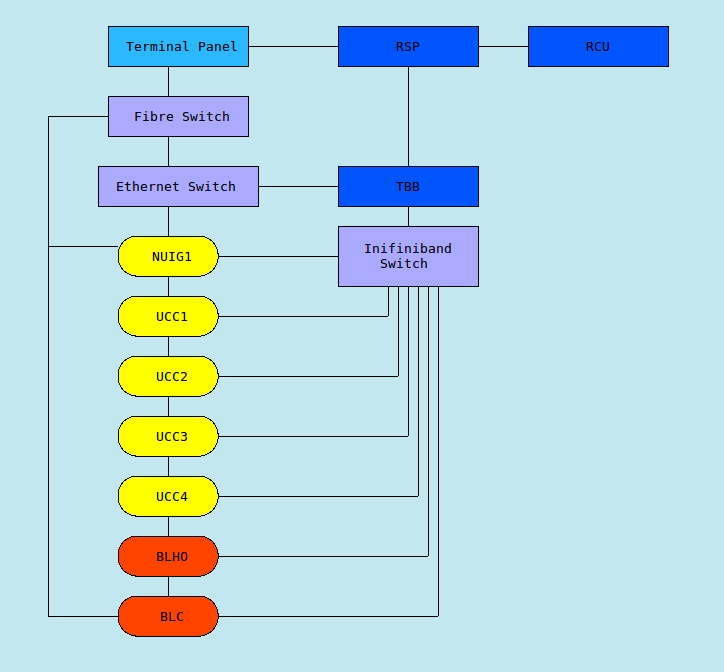
\includegraphics[width=10cm, height=12cm]{LOFAR.png}
    \caption{Diagram of I-LOFAR computer system structure}
    \label{fig:super}
\end{figure}

At the time of the writing of this user guide, the Breakthrough Listen computer system has been installed, and is shown in the diagram, operation and usage of breakthrough listen head node and node are not covered in this guide. Resources with greater descriptions on individual components of I-LOFAR are provider in section nine.

\section{REALTA Layout}
\todo[size=\small, color=green!20]{I assumed no previous knowledge of shell/Linux, as I know most students are taught python on a windows machine, let me know if you think I explain too much.}%
REALTA, is a Linux like system, therefore normal bash commands can be used to navigate the system. This section assumes that access to REALTA via a white-listed IvP4 has been obtained, and therefore a user name and password, alias as described in section two are also used. First from your home terminal ssh into the gateway, where lgc is an alias for username@160.6.237.10.

\vspace{3mm}

\verb|$ ssh lgc|

\vspace{3mm}

From this gateway we can ssh into nodes (nuig1, ucc1, ucc2 and ucc4). Please note that  nodes can only be accessed from this gateway, it is not possible to ssh from one processing node to another. If unsure of current working directory the command pwd will print out the current directory that the user is in. Next ssh into one of the data processing nodes for this example use ucc2.

\vspace{3mm}

\verb|$ ssh ucc2|

\vspace{3mm}

The command below will ssh into your sub-folder, scripts should be stored here, it is also possible to store a small amount of data. Be very careful as there is a limited amount of space, only keep data in a personal subfolder, if the desired data can not be located elsewhere on the system.

\vspace{3mm}

\verb|$ cd /mnt/ucc2_data1/data/yourusername|

\vspace{3mm}

All data processing and running of scripts should take place in ucc2 data1, if running a script outside a personal directory please consider where the output files are going, later in this section I have discussed the running of scripts and how to redirect the output to a personal sub-folder. As this is your own directory you can make directories and files as you see fit.

\vspace{3mm}

\verb|$ mkdir first_directory|
\bigbreak{}
\verb|$ nano first.file|

\vspace{3mm}

Two useful bash commands for managing files are cp and mv. The first command copies the input file and places the output file in the specified directory. The second moves the original file into the specified directory. Please note if you are copying a file from outside your directory, to your own directory please use cp instead of mv. If moving the file inside a personal directory,the output path can be greatly simplified.
\vspace{3mm}

\verb|$ cp input.file /mnt/ucc2_data1/data/yourusername|

\vspace{3mm}
Many different languages can be used to write scripts, but beware in order for the script to be executable a "shebang" must be used. A "shebang" line indicating the language that the script is written in, this must be at the top of the script. Scripts can be created and run using standard bash commands, for example running the a script called script.file.

\vspace{3mm}

\verb|$ source script.file|

\vspace{3mm}

Scripts can be run in any directory in a data processing node, but please be careful if running scripts outside a personal sub-folder. In order to view graphs that are outputted by your script, an x server can be used to generate a display window. First make sure that your current operating system has an x server installed, I personal use x11. In order to use a display window you need to add -x to both ssh commands for example,

\vspace{3mm}

\verb|$ ssh -X lgc|
\bigbreak{}
\verb|$ ssh -X ucc2|

\vspace{3mm}

The command xeyes can be used to test if a display window is available in lgc. After ssh into (ucc2), test if a display window is available using the commands

\vspace{3mm}

\verb|$ gnuplot|
\bigbreak{}
\verb|$ test|

\vspace{3mm}

If your preferred language is python, python scripts can be used. In general it is far more useful to try write as many scripts as possible in shell. There are many very useful bash packages which can be used as alternatives to the most used python packages. For example Gnuplot is a very useful plotting software, installed on REALTA, and is easy to use.

\vspace{3mm}

\verb|$ gnuplot|
\bigbreak{}
\verb|$ set xlabel "x axis"|
\bigbreak{}
\verb|$ set ylabel "y axis"|
\bigbreak{}
\verb|$ title"first plot"|
\bigbreak{}
\verb|$ plot sin(x)|
\vspace{3mm}



\section{Using Dockers}
When data processing in REALTA there are many useful software installed in order to simplify matters. Many of these software are installed on dockers. Docker is a set of platforms, that delivers software in packages called containers. Containers are isolated from one another and bundle their own software. You can use a docker by running the following generic command,

\vspace{3mm}

\verb|$ docker run -v host/directory:/container/directory|

\vspace{3mm}


This command will let the user mount a container, which contains the desired processing software to a file, which contains the data to be processed. The flag -v creates a volume, which are the preferred mechanism for persisting data generated by and used by docker containers. Other useful flags that should be used when using dockers are,

\vspace{3mm}

\verb|$ docker run --rm -it -v host/directory:/container/directory|

\vspace{3mm}


The flag --rm is important as it will close the docker after use, if --rm is not used the docker with keep running even after the user has exited the docker. If this happens multiple dockers can be left running on REALTA. To view all the current dockers that are running use the command docker ps. A word of warning many other user could possible be running dockers, so take care, for this reason its better to use –rm flag so you don’t have to worry about closing dockers after you have finished with them. 

When mounting containers to files it is advisable to define as general a mount as possible. The following command mounts to home local, which allows the user to access all directories in home local while inside the docker.

\vspace{3mm}

\verb|$ docker run -it –rm -v /mnt:/mnt -v /home:/home_local “container”|

\vspace{3mm}


Please note that a container name must be inserted in place of “container” in the above command. When inside the docker, the user can cd into other directories, and run scripts. If the data that you wish to process is in a personal directory after running the docker command, simply run the script as normal. If the data is in another directory in a processing node, cd into that directory run the script, making sure to direct the output back to a personal subfolder. If the data is in another node, a path must be defined to the data inside your script. This script can then be run inside your personal subfolder, where the output of that script should be stored. Multiple files can be mounted to a container at the same time, multiple containers can also use the same volume at the same time. It is also important to note that any file created while inside the docker, can only be edited inside that docker. Further information on dockers can be found in section nine.


\section{Useful Commands}
There are many useful bash commands that can greatly speed up data processing, and avoid the use of lengthy python scripts. With REALTA, data files can be very large, and take many different forms, possibly composed of many different columns. Each bash command listed below can be used to manipulate files in order to carry out data processing in a timely manner. Furthermore all of these commands can be piped together.
\vspace{3mm}

\noindent1.) Tail
\vspace{3mm}

\noindent Tail can be used to skip lines in a file, which is very handy for removing headers, the command below skips the first line of the input file. 

\vspace{3mm}

\verb|$ tail -n+2 input.file > output.file|

\vspace{3mm}
\noindent Tail can be used to print the last “n” number of lines in a file. The command below prints the last three lines in file file.txt. A plus symbol can be inserted in place of the minus symbol to give the first three lines of file.txt. If you wanted to use multiple files you can add the flag -q. By default the command tail followed by a file name will output the last ten lines of a file. 
\vspace{3mm}

\verb|$ tail -n 3 input.file > output.file|

\vspace{3mm}
\vspace{3mm}
\noindent2.) Cat
\vspace{3mm}

\noindent The command cat can be used to view the context of a single file or multiple files. The command cat followed by the file to read works for convectional file formats, niche file types that are generated while processing data in REALTA might need to be opened in a different way. For example filterbank files and timeseries file can't always be opened with cat only, the command below could be used instead,  
\vspace{3mm}
\todo[inline, color=green!20]{seem to have a problem inputting pipes}%

\verb|$ cat filename | od -f |

\vspace{3mm}
\noindent The od command in Linux is used to convert an input file into octal format, the flag -f converts to floats. Another useful function of cat is to combined files into one large file, the below command works on many file formats, this can be done as follows,
\vspace{3mm}

\verb|$ cat input1.file input2.file > output.file|

\vspace{3mm}
\noindent3.) Head
\vspace{3mm}

\noindent The command head can be used to view the header of a file, this command works for many file formats, for more niche file formats, that can be generated during data processing a header command from a specialised processing program may be needed. For example filterbank and timeseries files, that are produced using sigproc, which is a pulsar processing program. For these files the sigproc command header will need to be used instead.
\vspace{3mm}

\verb|$ head input.file|

\vspace{3mm}


\noindent4.) Grep
\vspace{3mm}

\noindent The command grep can be used for searching a file for either a word, or string. The following command looks for the word “cat” in the the file file.txt.

\vspace{3mm}

\verb|$ grep “cat” file.txt|

\vspace{3mm}
\noindent5.) Awk
\vspace{3mm}

\vspace{3mm}

\noindent The command awk can be used to print columns of a file or extract columns. The first command prints the first column of a file, and creates a new file with only the first column. The command below can be used both if a file containers headers, but also when headers aren't present.

\vspace{3mm}\vspace{3mm}

\verb|$ awk '{print $1}' input.file > output.file|

\vspace{3mm}

\noindent If a file has two columns of with headers 1 and 2, and you wanted to create a new file with only values in the first column that where greater then four but less then one hundred, the following could be used,
 
\vspace{3mm}

\verb|$ awk  '($1 > 8)  && ($1 < 100)' input.file > output.file|

\vspace{3mm}

\noindent The command below pipes together three different commands, this can make searching, sorting and getting desired values for data processing easy. The command below is an example of piping where dollar sign 1 means first column, dollar sign 2 means second column, and  dollar sign 0 means all columns. The sort -g sorts numerically (rather than alphabetically) -r means reverse order and -k2 means second column. In the command below, awk ignores header, and values in the third columns that are less then 8000, the values are then sorted, and the top 10 values are printed.

\vspace{3mm}

\verb|awk 'NR!=1{if ($3<8000) print $0}' input.file | sort -gr -k4 | head -10|

\vspace{3mm}

\noindent6.) Sed
\vspace{3mm}

\noindent Sed can be used to replace word, numbers or patterns in a file. The following command replaces the word one with the word two.
\vspace{3mm}

\verb|$ sed  's/one/two/' input.file|

\vspace{3mm}

\noindent7.) Uniq
\noindent The uniq command can be used to remove duplicate lines in a file for example,
\vspace{3mm}

\verb|$ uniq input.file|

\vspace{3mm}
\noindent Adding the flag -c will print the amount of times the line was repeated, the flag -d will print the repeated lines.
\todo[inline, color=green!20]{Should more complex/niche commands be included here or maybe another section?}%



\section{Observing with REALTA}

\todo[inline, color=green!20]{This section could be added to, if I get to observe}%
Before observing, an observation script must be written, which contains information specifying starting parameters, pointing, and recording preferences. Observation scripts can be run in ucc1, after observing the data gathered can be transferred to the relevant processing nodes. Observing with I-LOFAR is quite easy, and a standard script as shown below needs little adjustments. Before writing an observing script it is important to properly choose targets. For example, is the target visible from Birr, how bright is the target, does the target rise high enough and for long enough? 

In regards to the brightness and elevation of a target, it is important to note that the projected area of a LOFAR station is different with zenith angle, as the arrays are stationary. Therefore if you are offset by an angle, the length would appear to be shortened by a factor of cosine(zenith). Considering this we might need a dim target to rise to at least a forty-five degree elevation for a considerable time. After choosing a suitable target an observing script can be written. The first block consists of general parameters, these parameters normally don’t need to be changed for different targets. Important things to note in this first block are, the swlevel which refers to the software level of the station. The control processes of a LOFAR station are organized into six level. The first three levels are used in local mode when the telescope is observing as a lone system, the last three levels are used when the station is observing as a network, with the other LOFAR stations across Europe.

After changing software level, the script has to wait for a register update (rspctl) to complete. In summary, beam forming requires software level three, while usage of the RCU, RSP boards, and TBBs only requires software level two. All processes of the levels below the current level are also available to the user.


\vspace{7mm}

\verb|echo ‘initialising: SWLEVEL 2’|
\bigbreak{}
\verb|eval swlevel 2|
\bigbreak{}
\verb|rspctl  --wg=0|
\bigbreak{}
\verb|sleep 1|
\bigbreak{}
\verb|rspctl --bitmode=8|
\bigbreak{}
\verb|rspctl --bitmode|
\bigbreak{}
\verb|sleep 1|
\bigbreak{}
\verb|killall beamctl|
\bigbreak{}
\verb|sleep 3|
\bigbreak{}
\verb|echo ‘initialising: SWLEVEL 3’|
\bigbreak{}
\verb|eval swlevel3|
\bigbreak{}
\verb|sleep2|
\bigbreak{}
\verb|rspctl --splitter=0|
\bigbreak{}
\verb|sleep 3|
\bigbreak{}
\verb|rcus=’0:83,86:191|

\vspace{7mm}

The next block is the pointing block, the first command gives the pointing coordinates, the second command specific the beamforming. LOFAR carries out beamforming by converting equatorial coordinates to complex beamformer weights, digital and analogue beam pointing directions are updated with regular intervals. The pointing coordinates need to be correctly inputted in radians. 


\vspace{7mm}
\verb|pointing="RA(rad(-pi/2,pi/2)),DEC(rad(-pi/2,pi/2)),J2000"|
\bigbreak{}
\verb|beamctl --antennaset=HBA_JOINED --rcus=$rcus --band=110_190  --beamlets=0:487|
\bigbreak{}
\verb|--subbands=12:499 --anadir=$pointing --digdir=$pointing &|
\bigbreak{}
\verb|bash sleepuntil.sh YYYYMMDD HHMMSS.0|
\bigbreak{}
\verb|killall -9 beamctl|
\bigbreak{}
\verb|swlevel 0|

\vspace{7mm}

For example if you wanted to observed the pulsar PSR J0250+5854, with ICRS coordinates 02 50 17.78 +58 54 01.3, the pointing command would read,

\vspace{3mm}

\verb|pointing='0.7430579301269316,1.0280052319831219,J2000'|

\vspace{3mm}



The last block that is needed in an observing script is the recording block. The observing start and end time must be inputted by the user, a target name must be added, which can be anything the user chooses. For example if a you wanted observing to start at four in the morning on first of the July in the year 2020, the observing start command would read,

\vspace{3mm}

\verb|obs_start="2020-07-01T04:00.00.0"|

\vspace{3mm}

The sleepunitl.sh time should be set to a few minutes before the observation starts. The remainder of the scripts does not normally need to be changed.
\todo[inline, color=green!20]{should I add more details on commands used in scripts?}%

\vspace{7mm}

\verb|obs_start="YYYY-MM-DDTHH:MM:SS.0|
\bigbreak{}
\verb|obs_end="YYYY-MM-DDTHH:MM:SS.0"|
\bigbreak{}
\verb|target="name"|
\bigbreak{}
\verb|bash sleepuntil.sh YYYYMMDD HHMMSS|
\bigbreak{}
\verb|starts|
\bigbreak{}
\verb|echo $target $obs_start $obs_end|
\bigbreak{}
\verb|logdate=`date +"%Y%m%d%H%M%S"`|
\bigbreak{}
\verb|bash generic_ucc1_timestamps.sh $obs_start $obs_end 'dump_udp_ow_12' $target 2>&1 |
\bigbreak{}
\verb|tee -a $logdate'_$target.log'|

\vspace{7mm}

In section nine the LOFAR cookbook is linked, which gives great details, on flags used when observing.

\section{Data Processing}
\todo[inline, color=green!20]{Will probably add example based around task 3, would like to included an example on processing in relation to solar data, as I-LOFAR does a lot of that}%

This section demonstrates examples of data reduction, with the aim of providing the user with an idea of how to process different types of data on REALTA. The usage of individual software used in the examples or analysis of results are not covered in detail in this manual. The first two examples use a software called sigproc, which is installed on REALTA, in containers. Sigproc is a pulsar data processing software, but can also be used for fast radio bursts (FRB). The first data reduction exercise uses filterbank file (.fil), that was recorded by Parke. 

For our purpose a filterbank file can be thought of as an array of bandpass filters that separates the input signal into multiple components. We can located the filterbank files that we will be using in  /mnt/ucc2 data1/data/dmckenna/SMC. If you cd into this directory you can see that there are thirteen files labeled 1-D. Each .fil file corresponded to a different beam, which points at a different location in the sky. In the first diagram below we can see the beam layout, in the second we see the beam projection on the sky.

\vspace{7mm}

\begin{figure}[!tbp]
  \centering
  \begin{minipage}[b]{0.4\textwidth}
    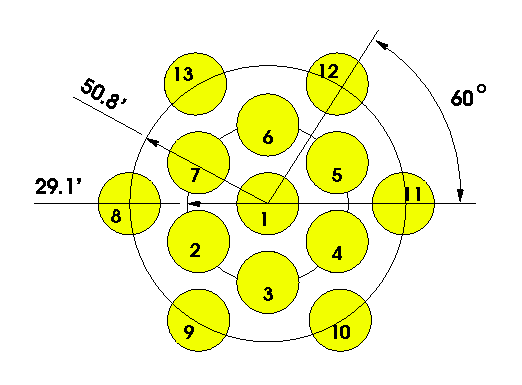
\includegraphics[width=\textwidth]{beam1.png}
    \caption{Beam Layout}
  \end{minipage}
  \hfill
  \begin{minipage}[b]{0.4\textwidth}
    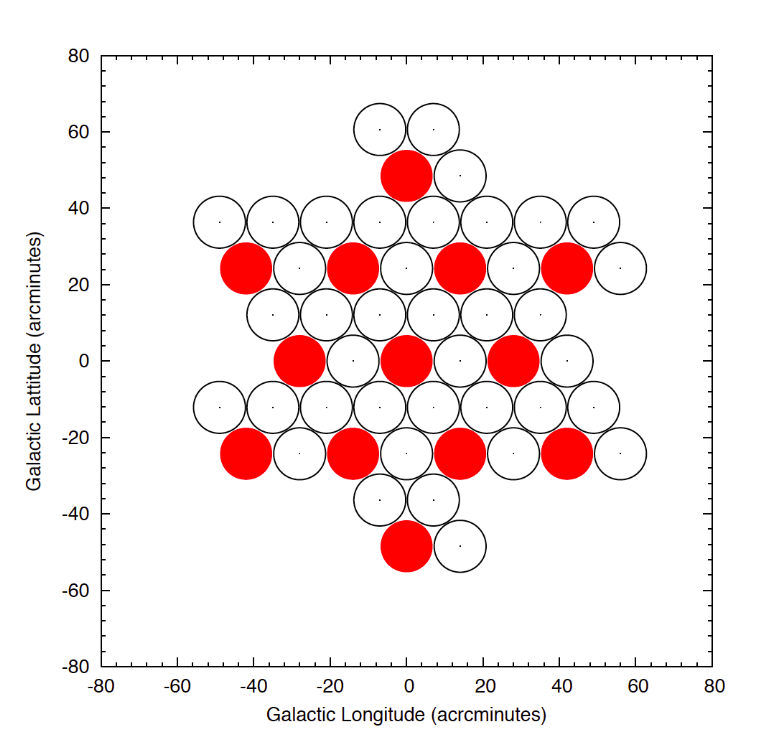
\includegraphics[width=\textwidth]{beam2.png}
    \caption{Beam Projection}
  \end{minipage}
\end{figure}

\vspace{70mm}


In order to use sigproc, we need to use a container that has sigproc installed, we will use the container pulsar-gpu-dsp2020 for this exercise. The container needs to be mounted to the data file, in order to process the data using sigproc commands, but first a data processing script should be created in a personal subfolder. The simple script shown below will first dedisperse each of the thirteen files for a range of dispersion measurements. Dedispersion is the process by which a filterbank file is corrected for the effects of interstellar dispersion, by the the interstellar medium. The dispersion measurement depend on both the electron density and distance between the target and the observer. Normally a range of dispersion measurements are used, as the correct value is often unknown. The command dedisperse will output time series files, the script below will output five hundred of these files for each beam. For example the outputted time series file,

\vspace{3mm}


\verb|"SMC021_008A1.2.tim"|

\vspace{3mm}


This file is a  time series file for the beam A, that has undergone a trial dedispersion of 2. 

\vspace{3mm}

\begingroup\makeatletter\def\@currenvir{verbatim}
\verbatim
#!/bin/sh

for file in  1 2 3 4 5 6 7 8 9 A B C D; do echo  
        for DM in {0..500}
        do 
                dedisperse "SMC021_008""$file""1.fil" -d $DM > 
                /mnt/ucc2_data1/data/personal_subfolder/
                "SMC021_008""$file""1.""$DM"".tim"
                seek "SMC021_008""$file""1.""$DM"".tim" -fftw -pulse -s  > 
                /mnt/ucc2_data1/data/personal_subfolder/
                "SMC021_008""$file""1.""$DM"".pls"
                rm "SMC021_008""$file""1.""$DM"".tim"
                rm "SMC021_008""$file""1.""$DM"".prd"
                rm "SMC021_008""$file""1.""$DM"".hst"
                rm "SMC021_008""$file""1.""$DM"".top"

        done
done

\end{verbatim}

\vspace{3mm}
After dedisperse, a search command called seek is used, this commands carries out both a periodicity search and a single pulse search (-pulse). Spectrum files can also be outputted using the flag -s. The command rm is used to remove all files that are generated by the seek command, that won't be used in this exercise. It is always good practice to only keep necessary files in a subfolder. Also note that all files have been directed back to a personal subfolder.

The use of a tmux session is suggested, when scripts like the one above have a long run time. When inside a session, REALTA can be used as normal. After running the script the user can simply leave the session without closing it, which allows the script to run in the background. Create a session before running the script above using the following command,

\vspace{3mm}

\verb|$ tmux new -s first_session|

\vspace{3mm}

When inside the session, login into docker, and run the following command,

\vspace{3mm}

\verb|$ docker login|
\bigbreak{}
\verb|$ docker run -it –rm -v /mnt:/mnt -v /home:/home_local pulsar-gpu-dsp2020|

\vspace{3mm}


Please note that in order to run a docker, you must have a docker account. The above command preforms a very general mount, as described in section five. When inside the docker containing sigproc, the script which contains sigproc commands can be executed. Next cd into the directory containing the data, and run the script. After this script has finished you should see single pulse search files (.pls), and periodicity search files (.prd), in the personal directory, that was used in the script.

 You should observe that (.pls) files have five columns, the first is dispersion measurements, the third is time, and the fourth signal to noise. For this example we will create single pulse graphs, for each of the thirteen beams. Next, we need to sort and merge files, we want to combine all the (.pls) files for one beam together.  This can be accomplished by removing the headers using tail. Then merge all the .pls for each beam individually into one large file using the cat command. You should end up with thirteen files. 

\begingroup\makeatletter\def\@currenvir{verbatim}
\verbatim
#!/bin/sh


for DM in {0..500}; do echo  

                tail -n+2 "SMC021_008D1.""$DM"".pls" >> 
                "SMC021_finished.""$DM"".pls"
                cat "SMC021_finished.""$DM"".pls"  >> 
                "SMC021_008D1_finished.pls"
                rm "SMC021_finished.""$DM"".pls"
done

\end{verbatim}
Next we can use the awk command to extract the columns we want to plot. Its also important to remove background noise in order to properly observe the signal, for this exercise use a signal to noise value of six. You can use the awk command to only extract columns where the fourth column is greater then 6. You should end up with three .csv  files for each of the thirteen beams, which should be very easy to plot.

\begingroup\makeatletter\def\@currenvir{verbatim}
\verbatim

awk '{$4!>6 && $4!<100}'  SMC021_00811_finished.pls  >> SMC021_00811_finished.pls
awk '{print $1}'  SMC021_00811_finished.pls >>  DM.csv 
awk '{print $3}'  SMC021_00811_finished.pls >>  time.csv 
awk '{print $4}'  SMC021_00811_finished.pls >>  SN.csv

\end{verbatim}

Now plot the thirteen beam graphs separately using something like the script below. Examining the plots its clear that most plots look the same, with constant lines of radio frequency interference (RFI). Examining graphs for the beams 6, 7 and D a unique signal that is absent in the other graphs can be observed. This signal is the FRB, we can zoom in to view the (FRB), further analysis can be carried out on the signal to determine, the pulse duration, DM and SNR. 

\begingroup\makeatletter\def\@currenvir{verbatim}
\verbatim
 
#!/usr/bin/python

from glob import glob
import numpy as np
import matplotlib.pyplot as plt
import pandas as pd
import csv

x = []
y = []
z = []
with open('time.csv','r') as csvfile:
    plots = csv.reader(csvfile)
    for row in plots:
        x.append(int(float(row[0])))
      
with open('DM.csv','r') as csvfile:
    plots = csv.reader(csvfile)
    for row in plots:
        y.append(int(float(row[0])))
       
with open('SN.csv','r') as csvfile:
    plots = csv.reader(csvfile)
    for row in plots:
        z.append(int(float(row[0])))
  
graph = plt.scatter(x, y, c=z, s = .1, cmap=plt.cm.plasma)    
cb = plt.colorbar(graph)
cb.set_label('SN')
plt.xlabel("time")
plt.ylabel("DM")
plt.title("SMC021_008D1.fil")
plt.savefig('/place to save/final.png')
plt.show()

\end{verbatim}

\todo[inline, color=green!20]{should I add more analysis after?}%
\vspace{70mm}

\begin{figure}[!tbp]
  \centering
  \begin{minipage}[b]{0.4\textwidth}
    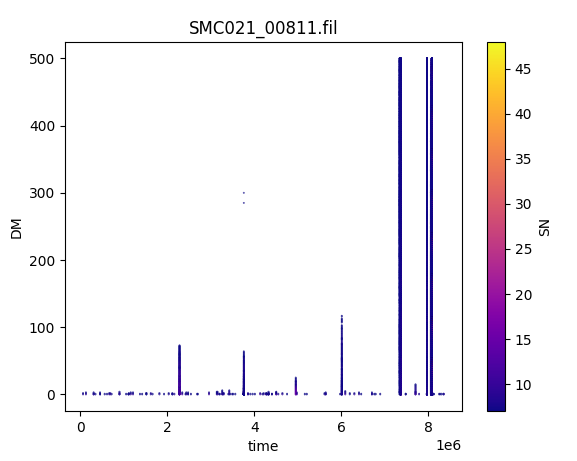
\includegraphics[width=\textwidth]{fil1.png}
    \caption{Beam 1 Graph}
  \end{minipage}
  \hfill
  \begin{minipage}[b]{0.4\textwidth}
    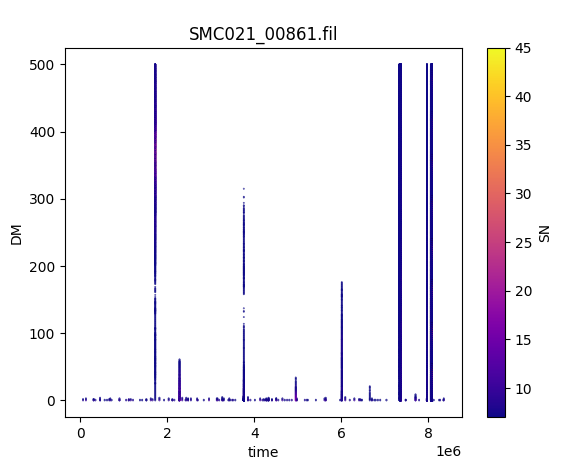
\includegraphics[width=\textwidth]{fil6.png}
    \caption{Beam 6 Graph}
  \end{minipage}
\end{figure}

\vspace{7mm}


\section{Resources}

Resources are divided into three section, the first gives resources for LOFAR, the second gives resources for useful bash data processing commands, the third gives useful astronomical software that can help with observational planning. Resources included in this section are scientific papers, user guide, tutorials, and blogs, all resources are inserted as links.
\todo[inline, color=green!20]{Would love to included list of containers, list section will hopefully be expanded further, would like to included more resources not related to pulsars}%
\vspace{3mm}

9.1 Section One (LOFAR resources)

\vspace{3mm}

\href{https://lofar.ie/wp-content/uploads/2018/03/station_data_cookbook_v1.2.pdf}{(station cookbook)}


\href{https://github.com/murphp30/I_LOFAR_workshop_2020}{(github tutorials for examples of data processing on users local machine)}


\href{https://old.astron.nl/radio-observatory/lofar-tools/lofar-calculators/lofar-calculators}{(LOFAR calculators)}


\href{https://lta.lofar.eu/Lofar}{(LOFAR long term archive)}


\href{https://www.lofar-surveys.org/gallery_preview.html}{(LOFAR image gallery)}


\href{http://www.astro.rug.nl/~peletier/BDT_LOFAR-IEEE_main.pdf}{(LOFAR architecture)}


\href{https://arxiv.org/pdf/1305.3550.pdf}{(LOFAR general overview)}


\href{https://docker-curriculum.com/}{(docker user guide)}


\href{https://docs.docker.com/storage/bind-mounts/}{(document on mounting containers to files)}


\vspace{3mm}
9.2 Section Two (bash commands)

\vspace{3mm}

\href{https://likegeeks.com/awk-command/}{(useful awk commands)}


\href{https://git-scm.com/book/en/v2/Git-on-the-Server-Generating-Your-SSH-Public-Key}{(generating public key)}


\href{https://linuxize.com/post/how-to-create-bash-aliases/}{(setting up alias)}


\href{https://www.web24.com.au/tutorials/use-grep-command-linux}{(using grep command)}


\href{https://www.geeksforgeeks.org/uniq-command-in-linux-with-examples/}{(using uniq)}


\vspace{3mm}

9.3 Section Three (astronomical resources)

\vspace{3mm}
\href{http://simbad.u-strasbg.fr/simbad}{(target search engine)}



\href{https://www.atnf.csiro.au/research/pulsar/psrcat/}{(pulsar catalogue)}


\href{http://sigproc.sourceforge.net/}{(pulsar data processing software SIGPROC)}


\href{http://sigproc.sourceforge.net/sigproc.pdf}{(SIGPROC user guide)}


\href{https://stellarium-web.org/}{(planetarium software)}

\section{Acknowledgements}
\todo[inline, color=green!20]{To be added later}%
\end{document}
